\section{Basic}
\inputcode{install vscode}{1_Basic/install_vscode.cpp}
\inputcode{default code}{1_Basic/default_code.cpp}
\inputcode{compare fuction}{1_Basic/cmp.cpp}
\inputcode{pbds}{1_Basic/pbds.cpp}

\section{Graph}
\inputcode{DFS 跟 BFS}{2_Graph/DFS_BFS.cpp}
\inputcode{Dijkstra}{2_Graph/Dijkstra.cpp}
\inputcode{Prim}{2_Graph/Prim.cpp}
\inputcode{正權找環}{2_Graph/PosCycle_Finding.cpp}
\inputcode{BellmanFord}{2_Graph/BellmanFord.cpp}
\inputcode{正權最大距離}{2_Graph/PosWeiMaxDistance.cpp}
\inputcode{負權最大距離}{2_Graph/NegWeiMaxDistance.cpp}
\inputcode{FloydWarshall}{2_Graph/FloydWarshall.cpp}
\inputcode{歐拉環與歐拉路}{2_Graph/EulerRoad.cpp}
\inputcode{Kosaraju 與拓樸 DP}{2_Graph/SCC_Topo_DP.cpp}
\inputcode{Tarjan 與 2-SAT}{2_Graph/2-SAT.cpp}
\inputcode{Planets Cycles}{2_Graph/Planets_Cycles.cpp}
\inputcode{Planet Queries II}{2_Graph/Planet_Queries_II.cpp}

\section{Data Structure}
\inputcode{BIT}{3_Data Structure/BIT.cpp}
\inputcode{DSU}{3_Data Structure/DSU.cpp}
\inputcode{Increasing Array Queries}{3_Data Structure/Increasing_Array_Queries.cpp}
\inputcode{線段樹}{3_Data Structure/Segment.cpp}
\inputcode{懶標線段樹}{3_Data Structure/LazySeg.cpp}
\inputcode{莫隊}{3_Data Structure/Mo.cpp}
\inputcode{Treap}{3_Data Structure/Treap.cpp}

\section{Flow}
\inputcode{Dinic}{4_Flow/Dinic.cpp}
\inputcode{MCMF}{4_Flow/MCMF.cpp}

\section{String}
\inputcode{KMP}{5_String/KMP.cpp}
\inputcode{Manacher}{5_String/Manacher.cpp}
\inputcode{Trie}{5_String/Trie.cpp}

\section{Math}
\inputcode{質因數分解}{6_Math/Prime.cpp}
\inputcode{矩陣快速冪}{6_Math/Fast_matrix.cpp}
\inputcode{盧卡斯定理}{6_Math/Lucas.cpp}
\inputcode{樹論分塊}{6_Math/Block.cpp}
\subsection{Mobius Theorem}

\begin{itemize}
\item 數論分塊可以快速計算一些含有除法向下取整的和式,就是像 $\sum_{i = 1} ^ {n} f(i) g(\left\lfloor\dfrac ni\right\rfloor)$ 的和式。當可以在 $O(1)$ 內計算 $f(r) - f(l)$ 或已經預處理出f的前綴和時,數論分塊就可以在 $O(\sqrt n)$ 的時間內計算上述和式的值。
\item 迪利克雷捲積 $h(x) = \sum_{d \mid x} f(d) g(\frac{x}{d})$
\item 積性函數
    \begin{itemize}
        \item 莫比烏斯函數
            \begin{enumerate}
                \item 定義
                $$ \begin{aligned}
                    \sum_{d \mid n} \mu (d)
                    &=
                    \begin{cases}
                        1 & \text{for } n = 1\\
                        0 & \text{for } n \neq 0
                    \end{cases}
                \end{aligned} $$

                \item $\mu$ 是常數函數 $1$ 的反元素\\
                $\Rightarrow \mu \ast 1 = \epsilon$,$\epsilon (n) \text{只在} n = 1 \text{時為 1,其餘情況皆為 0。}$
            \end{enumerate}

        \item $\phi$ 歐拉函數: $x$ 以下與 $x$ 互質的數量
        $$ \begin{aligned}
            \phi \ast 1
            &= \sum_{d \mid n} \phi(\dfrac {n}{d}) \ \ \text{質因數分解}\\
            &= \sum_{i = 0} ^ {c} \phi(p ^ i)\\
            &= 1 + p^0(p-1) + p^1(p-1) + ... + p^{c-1}(p-1)\\
            &= p^c\\
            &= id
        \end{aligned} $$
    \end{itemize}

\item 莫比烏斯反演公式
    \begin{itemize}
        \item $f(n)=\sum_{d\mid n}g(d)\Leftrightarrow g(n)=\sum_{d\mid n}\mu(d)f(\frac{n}{d})$
        \item $f(n)=\sum_{n\mid d}g(d)\Leftrightarrow g(n)=\sum_{n\mid d}\mu(\frac{d}{n})f(d)$
    \end{itemize}

\item 例子
$$ \begin{aligned}
    &\sum_{i = a}^{b} \sum_{j = c}^{d} [gcd(i, j) = k]\\
    &\Rightarrow \sum_{i = 1}^{x} \sum_{j = 1}^{y} [gcd(i, j) = k]\\
    &= \sum_{i = 1}^{\left\lfloor\dfrac {x}{k} \right\rfloor} \sum_{j = 1}^{\left\lfloor\dfrac {y}{k} \right\rfloor} \epsilon(gcd(i, j))\\
    &= \sum_{i = 1}^{\left\lfloor\dfrac {x}{k} \right\rfloor} \sum_{j = 1}^{\left\lfloor\dfrac {y}{k} \right\rfloor} \sum_{d \mid gcd(i, j)} \mu(d)\\
    &= \sum_{d = 1}^{\infty} \mu(d) \sum_{i = 1}^{\left\lfloor\dfrac {x}{k} \right\rfloor} [d \mid i] \sum_{j = 1}^{\left\lfloor\dfrac {y}{k} \right\rfloor} [d \mid j] \text{\ \ d 可整除 i 時為 1}\\
    &= \sum_{d = 1}^{min(\left\lfloor\dfrac {x}{k} \right\rfloor, \left\lfloor\dfrac {y}{k} \right\rfloor)} \mu(d) \left\lfloor\dfrac {x}{kd} \right\rfloor \left\lfloor\dfrac {y}{kd} \right\rfloor
\end{aligned} $$
\end{itemize}
\subsection{Catalan Theorem}
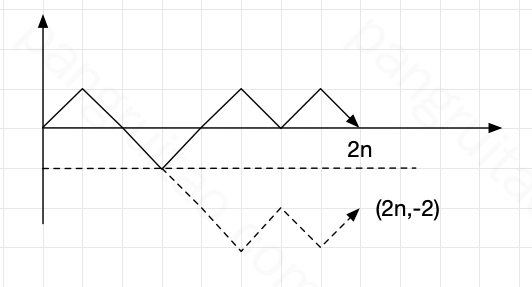
\includegraphics[width=8cm]{6_Math/Catalan.png}
\begin{enumerate}
\item $n$ 個往上 $n$ 個往下,先枚舉所有情況 $\frac{(2n)!}{n!n!} = C_{n}^{2n}$
\item 扣掉非法的,有多少種可能讓最後的點落在 $(2n, -2)$
\end{enumerate}
假設往上有 $x$ 個,往下有 $y$ 個,會有:
$$
\begin{cases}
x + y = 2n\\
y - x = 2
\end{cases}
\Rightarrow
\begin{cases}
x = n - 1\\
y = n + 1
\end{cases}
$$
所以只要扣掉 $C_{n-1}^{2n}$ 即可
\inputcode{莫比烏斯反演}{6_Math/Mobius.cpp}

\section{Search and Gready}
\inputcode{二分搜}{7_Search and Gready/Binary_Search.cpp}
\inputcode{三分搜}{7_Search and Gready/Triple_Search.cpp}

\section{Tree}
\inputcode{LCA}{8_Tree/LCA.cpp}
\inputcode{樹 DFS}{8_Tree/Tree_DFS.cpp}
\inputcode{樹重心}{8_Tree/Tree_Centroid.cpp}
\inputcode{節點距離總和}{8_Tree/Tree_Sum_Distances.cpp}
\inputcode{有權樹直徑}{8_Tree/Weighted_Tree_Distance.cpp}
\inputcode{樹壓平}{8_Tree/Tree_Compress.cpp}

\section{DP}
\inputcode{背包問題}{9_DP/Bag.cpp}
\inputcode{Bitmask DP}{9_DP/Bitmask_DP.cpp}
\inputcode{硬幣}{9_DP/Coin.cpp}
\inputcode{編輯距離}{9_DP/Edit_Distance.cpp}
\inputcode{LCS}{9_DP/LCS.cpp}
\inputcode{LIS}{9_DP/LIS.cpp}
\inputcode{Projects}{9_DP/Projects.cpp}
\inputcode{Removal Game}{9_DP/Removal_Game.cpp}
\inputcode{Max overlap}{9_DP/Max_overlap.cpp}

\section{Geometry}
\inputcode{Cross Product}{10_Geometry/Cross_Product.cpp}
\inputcode{Convex Hull}{10_Geometry/Convex_Hull.cpp}